%% Bookheader, Nov 8, 2020; July 18, 2022

\documentclass[11pt]{../Support/ourbook}
%% or for landscape, comment out line above and use this one:
%%\documentclass[landscape,11pt]{ourbook}

%% This will keep space from stretching around display math:

\makeatletter
\renewcommand\normalsize{%
   \@setfontsize\normalsize\@xipt{13.6}%
   \abovedisplayskip 11\p@  \@minus6\p@
   \abovedisplayshortskip \z@ 
   \belowdisplayshortskip 6.5\p@ \@minus3\p@
   \belowdisplayskip \abovedisplayskip
   \let\@listi\@listI}
\makeatother
\normalsize


\begin{document}

\tableofcontents
\graphicspath{{../../Chapters/falling_bodies/en_US}}
\chapter{Falling Bodies}

Because of gravity, if you throw a hammer straight up in the air, from
the moment it leaves your hand until it hits the ground, it is
accelerating toward the center of the earth at a constant rate.

\emph{Acceleration} can be defined as change in velocity. If the hammer leaves your
hand with a velocity of 12 meters per second upward, one second later
it will be rising, and its velocity will have slowed to 2.2 meters per
second. One second after that, the hammer will be falling at a rate of
7.6 meters per second. Every second the hammer's velocity is changing by
9.8 meters per second, and that change is always toward the center of
the earth. When the hammer is going up, gravity is slowing it down by
9.8 meters per second, each second it is in the air.  When the hammer is coming down,
gravity is speeding it up by 9.8 meters per second.\index{acceleration}
% Connect to vectors
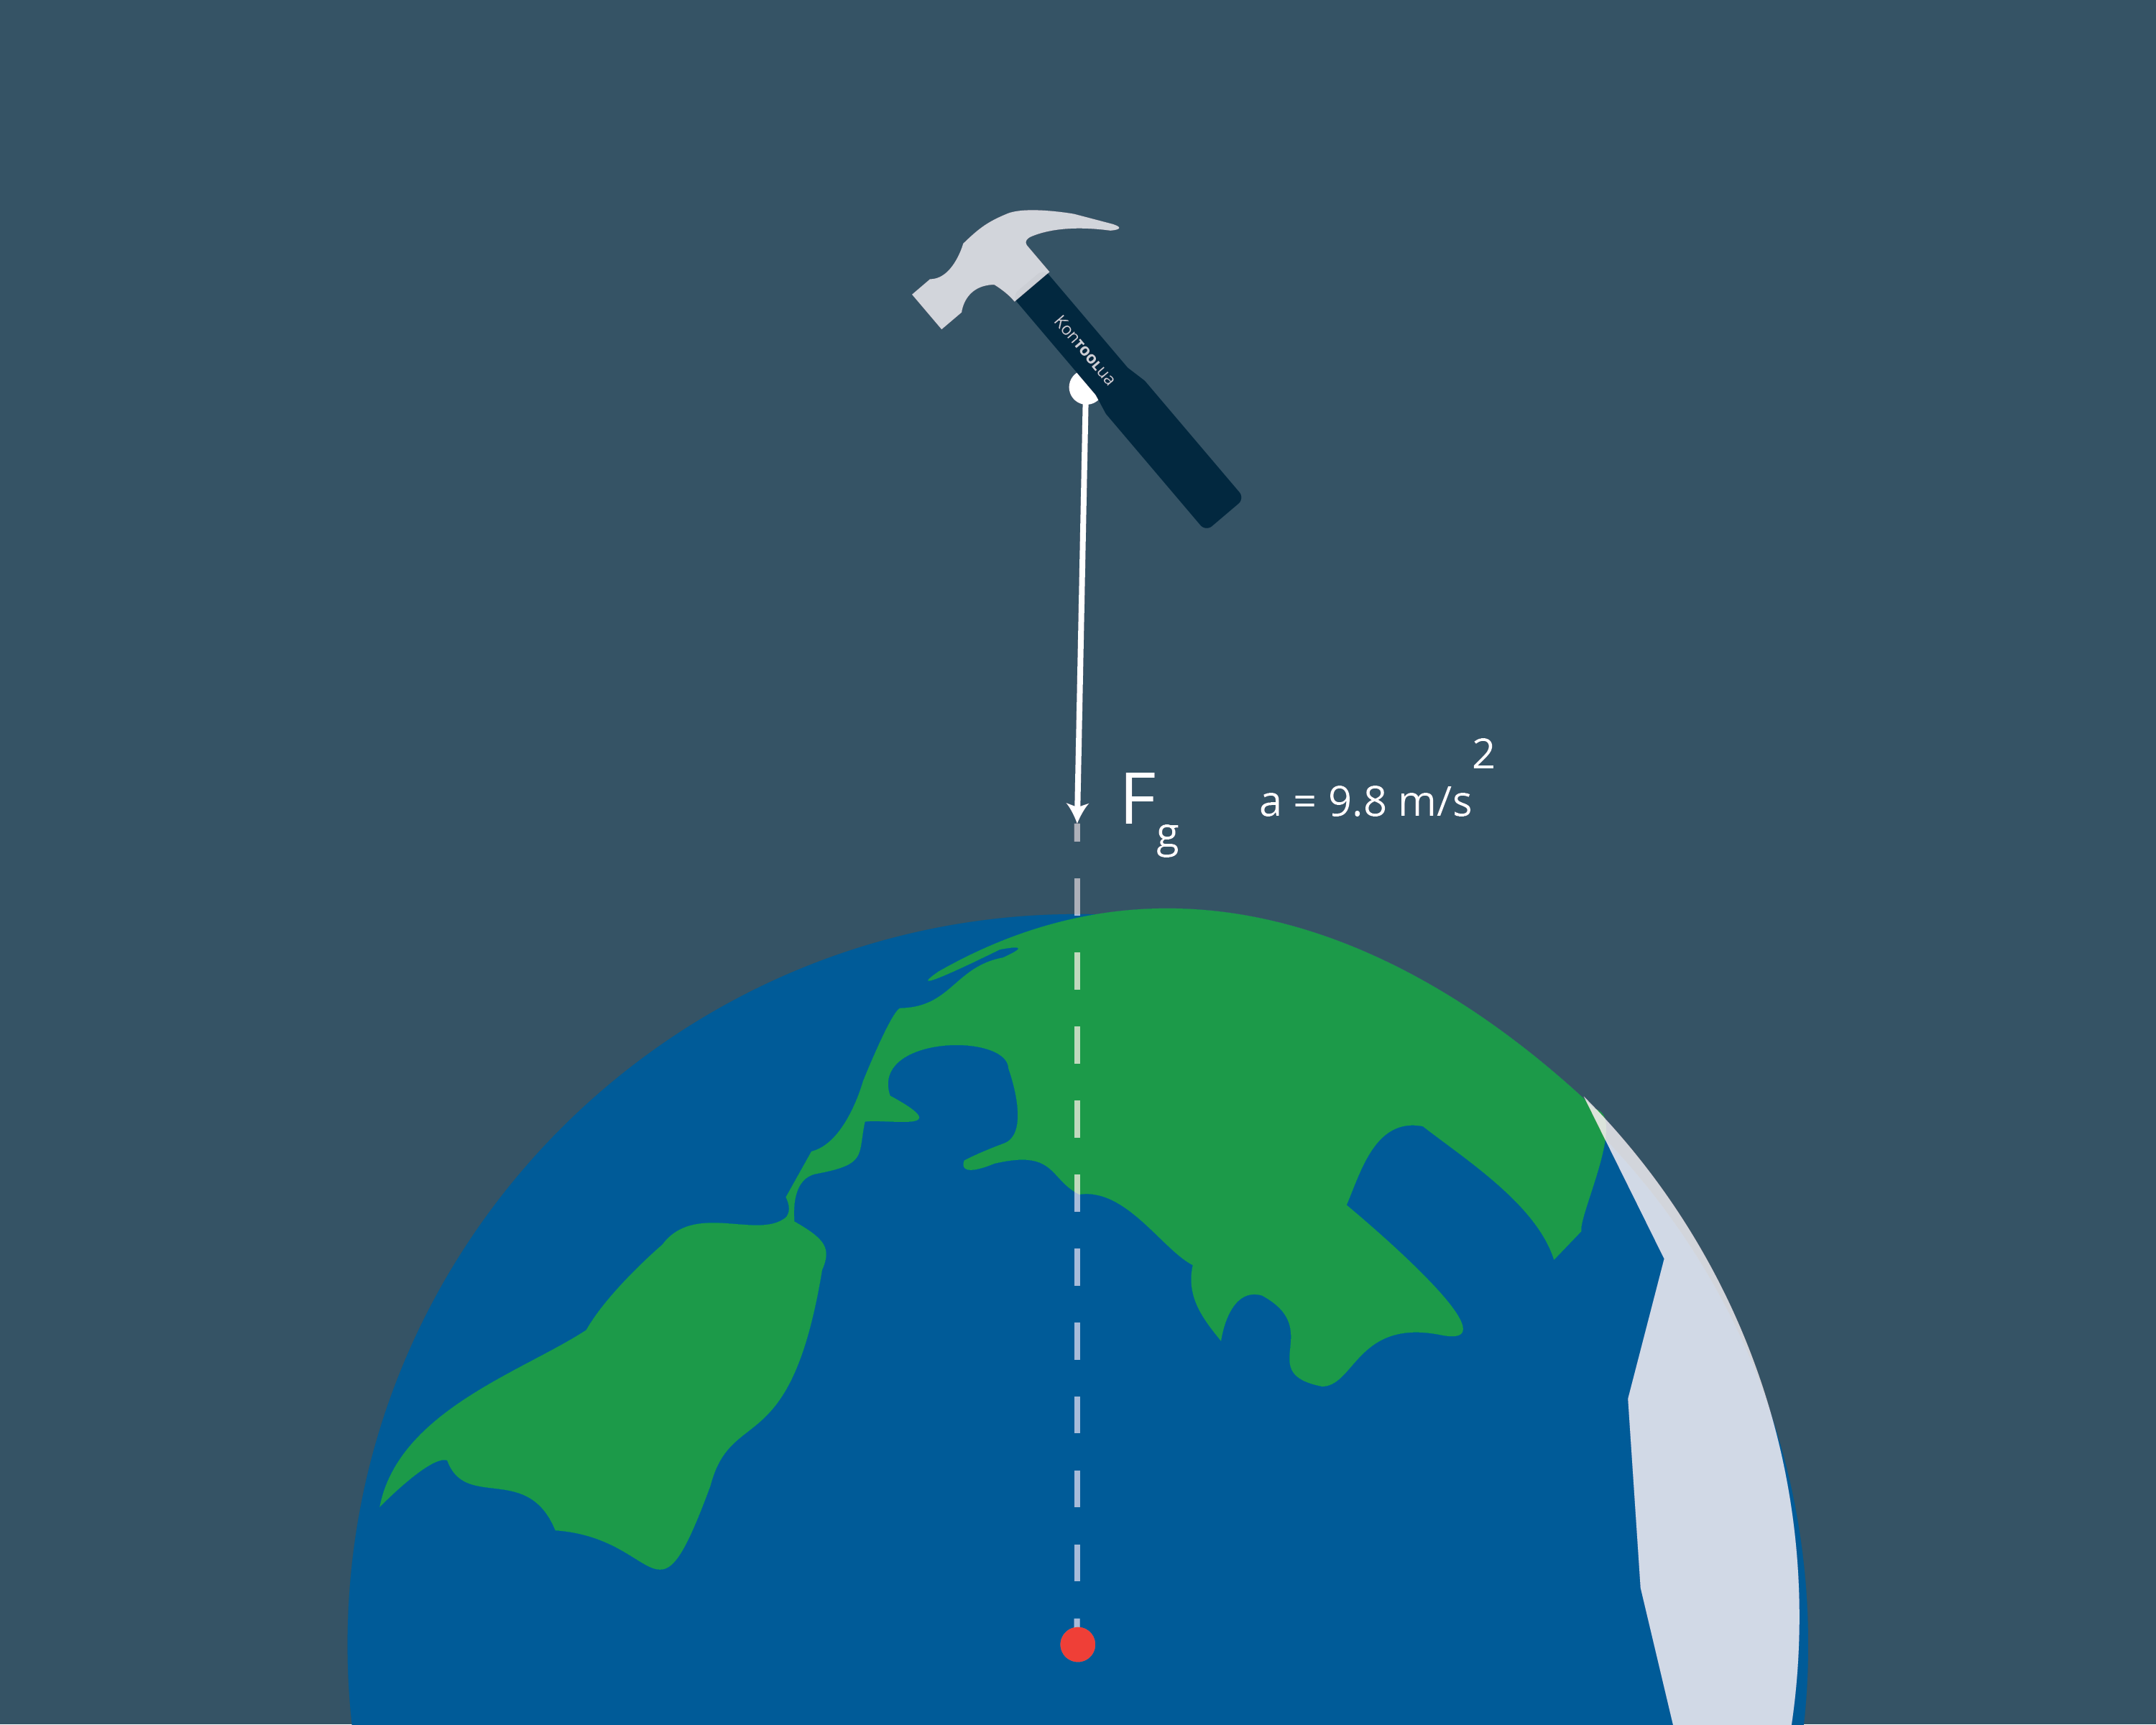
\includegraphics[width=1\textwidth]{hammerFall.png}


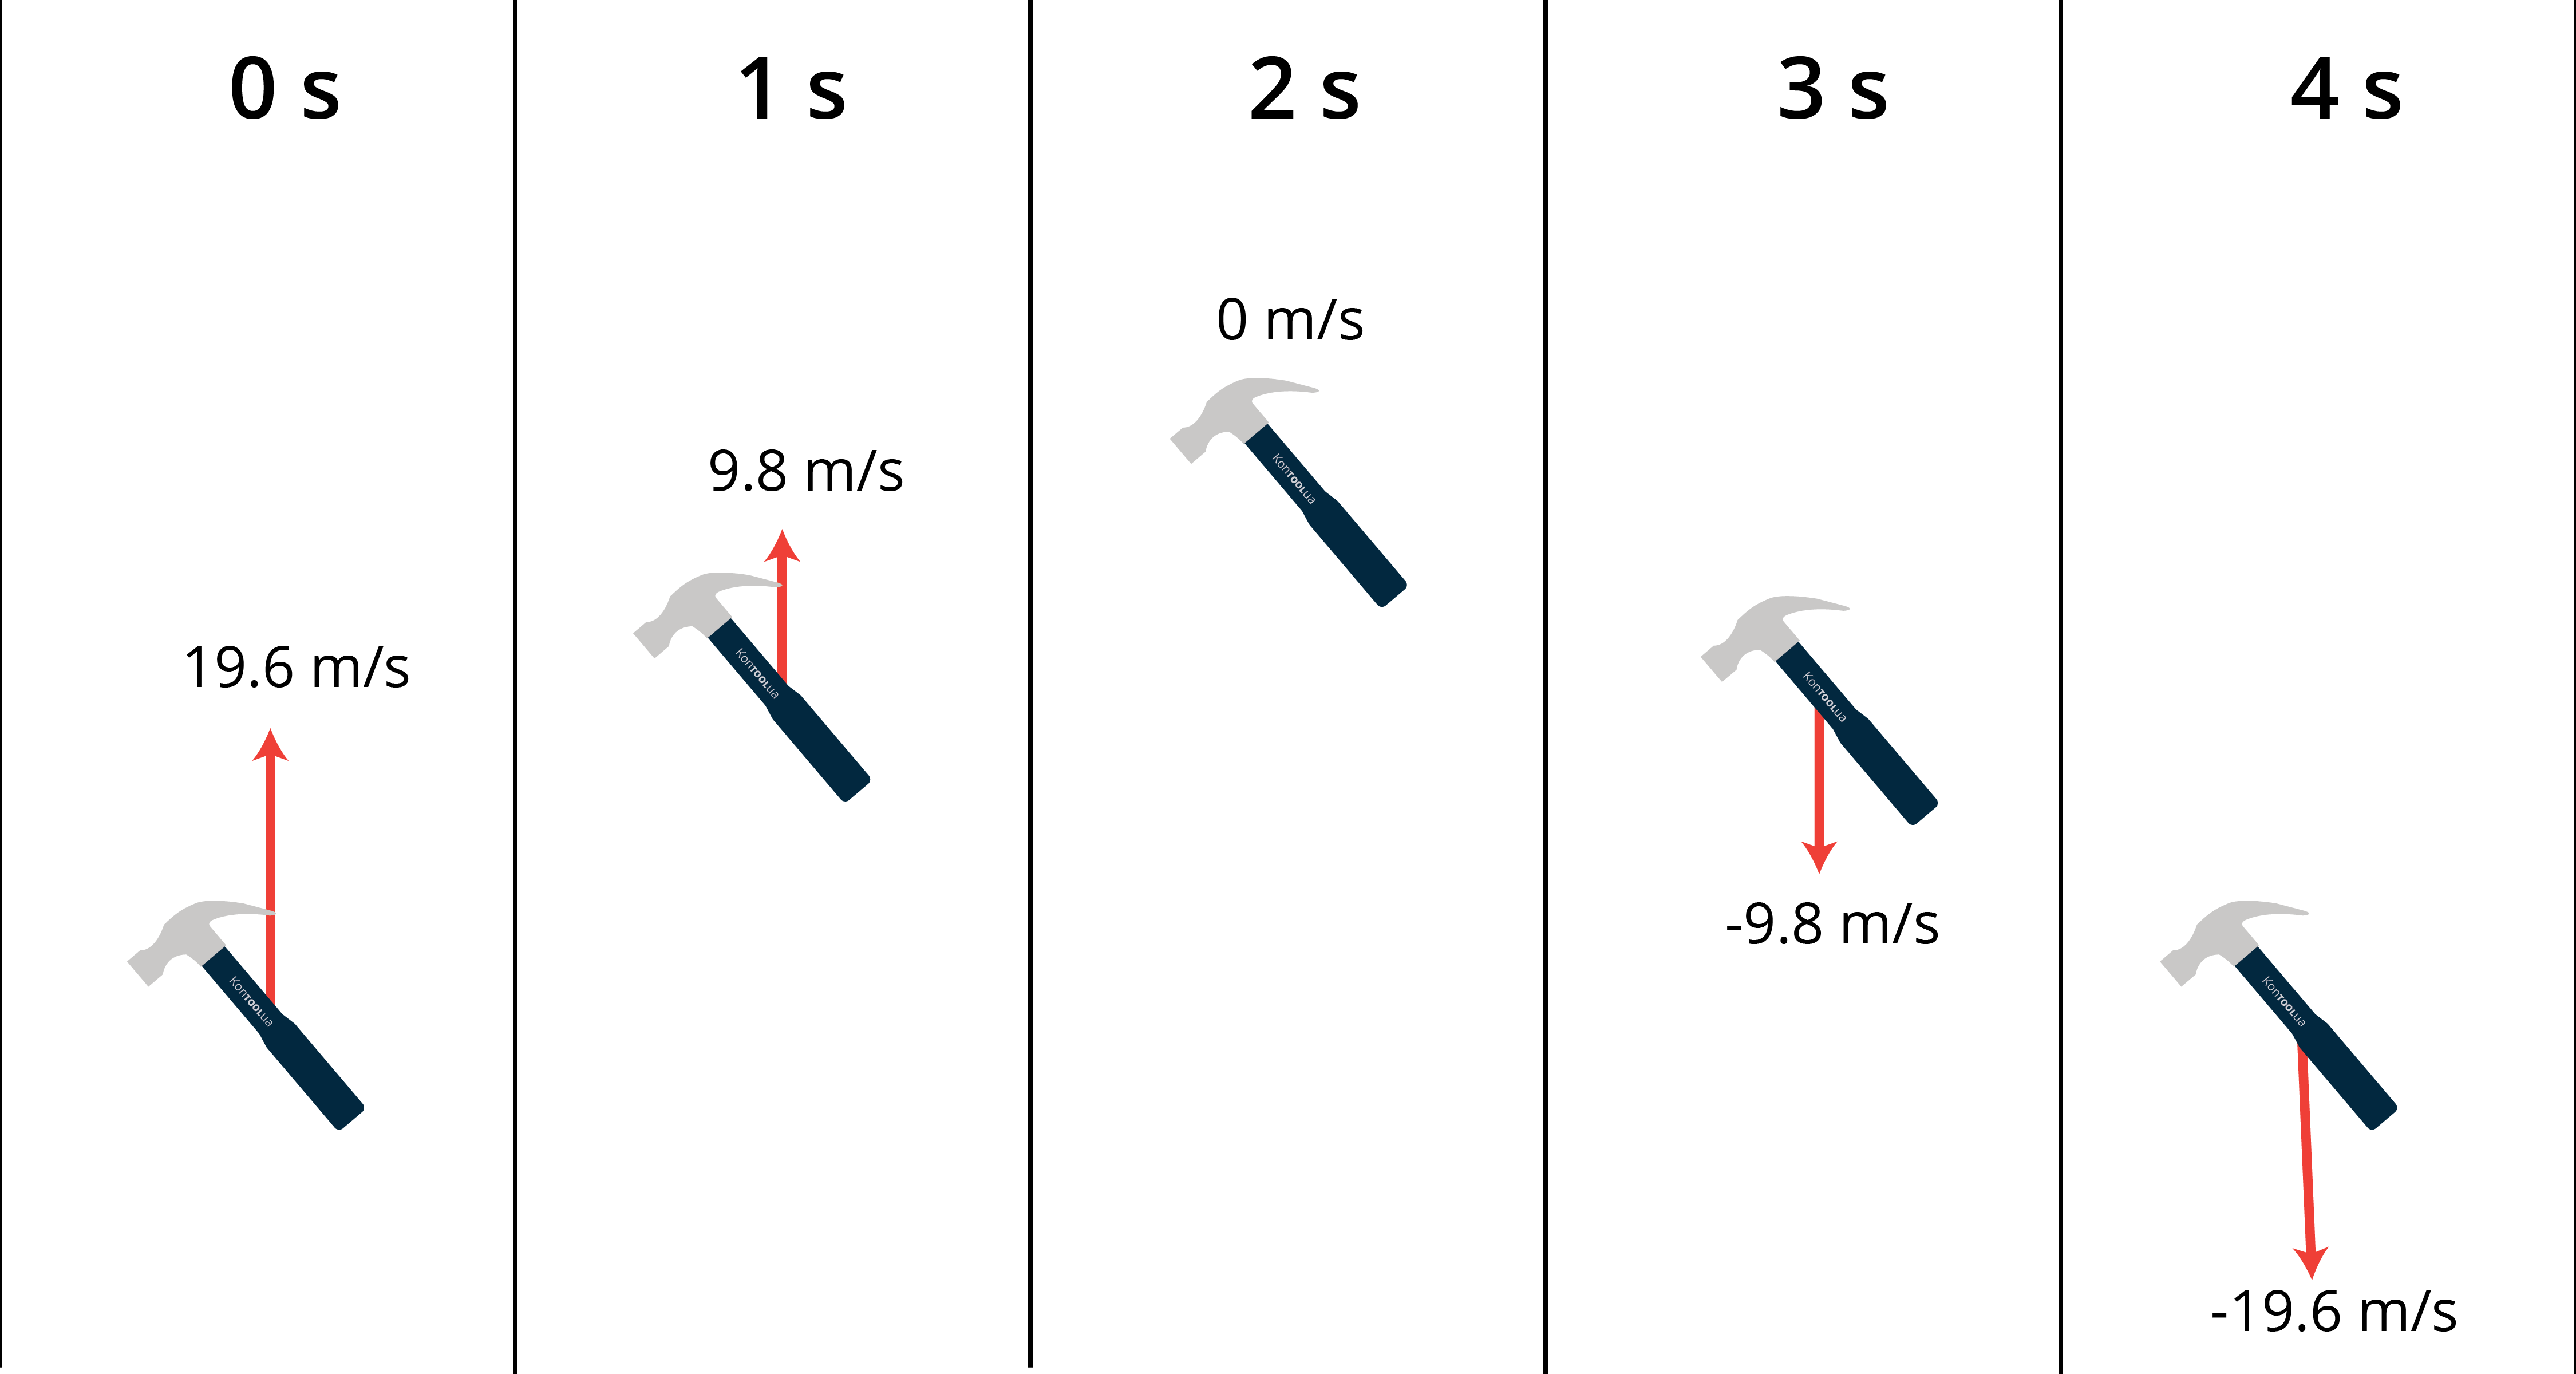
\includegraphics[width=1\textwidth]{hammerTime.png}

Acceleration due to gravity on earth is a constant negative 9.8 meters per second per second:
\begin{equation*}
a = -9.8   
\end{equation*}
(Why is it negative? We are talking about height, which increases as
you go away from the center of the earth. Acceleration is changing the
velocity in the opposite direction.)

\section{Calculating the Velocity}

Given that the acceleration is constant, it makes sense that the
velocity is a straight line. Assuming once again that the hammer
leaves your hand at 12 meters per second, then the upwards velocity at
time $t$ is given by:
\begin{equation*}
  v = 12 - 9.8t
\end{equation*}

Note that the velocity of the hammer is being given as a function. Here is its graph:

\begin{tikzpicture}
    \begin{axis}[
        xmin=-0.25,xmax=2.75,
        ymin=-13,ymax=13,
        axis x line=middle,
        axis y line=middle,
        axis line style=<->,
        xlabel={$t$},
        ylabel={$v$},
        ]
        \addplot[no marks,sdkblue] expression[domain=0:2.25,samples=100]{x * (-9.8) + 12} node[left] {$12 - 9.8t$}; 
    \end{axis}
\end{tikzpicture}

\begin{Exercise}[title={When is the apex of flight?}, label=vapex]
  Given the hammer's velocity is given by $12 - 9.8t$, at what time (in seconds)
  does it stop rising and begin to fall?
\end{Exercise}
\begin{Answer}[ref=vapex]
  Solve for when the velocity is zero.

  $t = \frac{12}{9.8} = 1.22$ seconds after release.
\end{Answer}

At this point, we need to acknowledge air resistance. Gravity
is not the only force on the hammer; as it travels through the air,
the air tries to slow it down. This force is called \emph{air resistance},
and for a large, fast-moving object (like an airplane) it is GIGANTIC force. For a
dense object (like a hammer) moving at a slow speed (what you generate
with your hand), air resistance doesn't significantly affect acceleration.
% Relate to f=ma

\section{Calculating Position}

If you let go of the hammer when it is 2 meters
above the ground, the height of the hammer is given by:
\begin{equation*}
  p = -\frac{9.8}{2}t^2 + 12t + 2
\end{equation*}

Here is a graph of this function:

\begin{tikzpicture}
    \begin{axis}[
        xmin=-1.2,xmax=3.5,
        ymin=-13,ymax=13,
        axis x line=middle,
        axis y line=middle,
        axis line style=<->,
        xlabel={$t$},
        ylabel={$p$},
      ]
      \addplot[no marks,sdkblue,dashed,<-] expression [domain=-0.7:0,samples=100] {(-4.9)*(x^2) + 12 * x + 2};
      \addplot[no marks,sdkblue] expression [domain=0:2.58,samples=100] {(-4.9)*(x^2) + 12 * x + 2};
      \addplot[no marks,sdkblue,dashed,->] expression [domain=2.58:3,samples=100] {(-4.9)*(x^2) + 12 * x + 2};
    \end{axis}
\end{tikzpicture}


How do we know? \textbf{The change in position between time
  $0$ and any time $t$ is equal to the area under the velocity graph
  between $x = 0$ and $x = t$.}

Let's use the velocity graph to figure out how much the position has
changed in the first second of the hammer's flight. Here's the
velocity graph with the area under the graph for the first second filled
in:

\usepgfplotslibrary{fillbetween}

\begin{tikzpicture}
    \begin{axis}[
        xmin=-0.25,xmax=2.75,
        ymin=-13,ymax=13,
        axis x line=middle,
        axis y line=middle,
        axis line style=<->,
        xlabel={$t$},
        ylabel={$v$},
      ]
      \addplot[no marks,sdkblue, name path=f] expression[domain=0:2.25,samples=100]{x * (-9.8) + 12} node[left] {$12 - 9.8t$};
      \path[name path=xaxis] (axis cs:0,0) -- (axis cs:1,0);
      \addplot[
        thick,
        color=sdkblue,
        fill=sdkblue, 
        fill opacity=0.05
    ]
    fill between[
        of=f and xaxis,
        soft clip={domain=0:1},
    ];
    \addplot[dashed,gray] coordinates {(0,12)(1,12)};
    \addplot[dashed,gray] coordinates {(1,12)(1,0)};
    \end{axis}
\end{tikzpicture}

The blue filled region is the area of the dashed rectangle minus that
empty triangle in its upper left.  The height of the rectangle is
twelve and its width is the amount of time the hammer has been in
flight ($t$). The triangle is $t$ wide and $9.8t$ tall. Thus, the
area of the blue region is given by $12t - \frac{1}{2}9.8 t^2$.

That's the change in position. Where was it originally? 2 meters off
the ground. So the height is given by $p = 2 + 12t - \frac{1}{2}9.8t^2$.
We usually write terms so that the exponent decreases, so:

$$p = - \frac{1}{2}9.8t^2 + 12t + 2$$

Finding the area under the curve like this is called
\textit{integration}. We say ``To find a function that gives the
change in position, we just integrate the velocity function.''  A lot
of the study of calculus is learning to integrate different sorts of
functions.\index{integration}

One important note about integration: Any time the curve drops under
the $x$-axis, the area is considered negative. (Which makes sense,
right? If the velocity is negative, the hammer's position is
decreasing.)


\begin{tikzpicture}
    \begin{axis}[
        xmin=-0.25,xmax=2.75,
        ymin=-13,ymax=13,
        axis x line=middle,
        axis y line=middle,
        axis line style=<->,
        xlabel={$t$},
        ylabel={$v$},
      ]
      \addplot[no marks,sdkblue, name path=f] expression[domain=0:2.25,samples=100]{x * (-9.8) + 12} node[left] {$12 - 9.8t$};
      \path[name path=xaxis] (axis cs:0,0) -- (axis cs:2.25,0);
      \addplot[
        thick,
        color=sdkblue,
        fill=sdkblue, 
        fill opacity=0.05
      ]
      fill between[
        of=f and xaxis,
        soft clip={domain=0:1.2245},
      ];
      \addplot[
        thick,
        color=red,
        fill=red, 
        fill opacity=0.07
      ]
      fill between[
        of=f and xaxis,
        soft clip={domain=1.2245:2.1},
      ];
    \end{axis}
\end{tikzpicture}


\section{Quadratic functions}

Functions of the form $f(x) = a x^2 + b x + c$ are called \newterm{quadratic functions}. 
If $a > 0$, the ends go up.
If $a < 0$, the ends go down.\index{quadratic functions}


\begin{tikzpicture}
  \begin{axis}[
      xmin=-2.2,xmax=1.2,
      ymin=-2,ymax=3,
      axis x line=middle,
      axis y line=middle,
      axis line style=<->,
    ]
    \addplot[no marks,sdkblue] expression [domain=-2:1,samples=100] {(2)*(x^2) + 2 * x - 1};
  \end{axis}
  \node[right] at (1,4) {$2x^2 + 2x - 1$};
\end{tikzpicture}
\hspace{4mm}
\begin{tikzpicture}
  \begin{axis}[
    xmin=-1.5,xmax=1.5,
    ymin=-2,ymax=1.5,
    axis x line=middle,
    axis y line=middle,
    axis line style=<->,
  ]
  \addplot[no marks,sdkblue] expression [domain=-1.5:1.5,samples=100] {(-1.2)*(x^2) + 0.5 * x + 1};
\end{axis}
\node[right] at (0.5,1) {$-1.2 x^2 + 0.5 x + 1$};
\end{tikzpicture}

The graph of a quadratic function is a \newterm{parabola}.

\section{Simulating a falling body in Python}

Now you are going to write some Python code that simulates the flying hammer. First, we are just going to print out the position, speed, and acceleration of the hammer for every 1/100th of a second after it leaves your hand. (Later we will make a graph.)

Create a file called \filename{falling.py} and type this into it:

\begin{Verbatim}
# Acceleration on earth
acceleration = -9.8 # m/s/s

# Size of time step
time_step = 0.01 # seconds

# Initial values
speed = 12  # m/s upward
height = 2  # m above the ground
current_time = 0.0  # seconds after release

# Is the hammer still aloft?
while height > 0.0:

    # Show the values
    print(f"{current_time:.2f} s:")
    print(f"\tacceleration: {acceleration:.2f} m/s/s")
    print(f"\tspeed: {speed:.2f} m/s")
    print(f"\theight: {height:.2f} m")

    # Update height
    height = height + time_step * speed

    # Update speed
    speed = speed + time_step * acceleration

    # Update time
    current_time = current_time + time_step


print(f"Hit the ground: Complete")
\end{Verbatim}

When you run it, you will see something like this:
\begin{Verbatim}
0.00 s:
	acceleration: -9.80 m/s/s
	speed: 12.00 m/s
	height: 2.00 m
0.01 s:
	acceleration: -9.80 m/s/s
	speed: 11.90 m/s
	height: 2.12 m
0.02 s:
	acceleration: -9.80 m/s/s
	speed: 11.80 m/s
	height: 2.24 m
0.03 s:
	acceleration: -9.80 m/s/s
	speed: 11.71 m/s
	height: 2.36 m
...
2.60 s:
	acceleration: -9.80 m/s/s
	speed: -13.48 m/s
	height: 0.20 m
2.61 s:
	acceleration: -9.80 m/s/s
	speed: -13.58 m/s
	height: 0.07 m
Hit the ground: Complete
\end{Verbatim}

Note that the acceleration isn't changing at all, but it is changing
the speed, and the speed is changing the height.

We can see that the hammer in our simulation hits the ground just
after 2.61 seconds.

\subsection{Graphs and Lists}

Now, we are going to graph the acceleration, speed, and height using a
library called matplotlib. However, to make the graphs, we
need to gather all the data into lists.\index{matplotlib}

For example, we will have a list of speeds, and the first three
entries will be 12.0, 11.9, and 11.8.\index{lists, python}

We create an empty list and assign it to a variable like this:
\begin{Verbatim}
x = []
\end{Verbatim}

Then we can add items like this:
\begin{Verbatim}
x.append(3.14)
\end{Verbatim}

To get the first time back, we can ask for the object at index 0.
\begin{Verbatim}
y = x[0]
\end{Verbatim}
Note that the list starts at 0.  So if you have 32 items in the list,
the first item is at index 0. The last item is at index 31.

Duplicate the file \filename{falling.py} and name the new copy \filename{falling\_graph.py}

We are going to make a plot of the height over time. At the start of the program, you will import the
matplotlib library.  At the end of the program, you will create a plot and show it to the user.

In \filename{falling\_graph.py}, add the bold code:

\begin{Verbatim}[commandchars=\\\{\}]
\textbf{import matplotlib.pyplot as plt}

# Acceleration on earth
acceleration = -9.8 # m/s/s

# Size of time step
time_step = 0.01 # seconds

# Initial values
speed = 12  # m/s upward
height = 2  # m above the ground
current_time = 0.0  # seconds after release

\textbf{# Create empty lists}
\textbf{accelerations = []}
\textbf{speeds = []}
\textbf{heights = []}
\textbf{times = []}

# Is the hammer still aloft?
while height > 0.0:

    \textbf{# Add the data to the lists}
    \textbf{times.append(current_time)}
    \textbf{accelerations.append(acceleration)}
    \textbf{speeds.append(speed)}
    \textbf{heights.append(height)}
    
    # Update height
    height = height + time_step * speed

    # Update speed
    speed = speed + time_step * acceleration

    # Update time
    current_time = current_time + time_step

\textbf{# Make a plot}
\textbf{fig, ax = plt.subplots()}
fig.suptitle("Falling Hammer")
\textbf{ax.set_xlabel("Time (s)")}
\textbf{ax.set_ylabel("Height (m)")}
\textbf{ax.plot(times, heights)}
\textbf{plt.show()}
\end{Verbatim}

When you run the program, you should see a graph of the height over time.

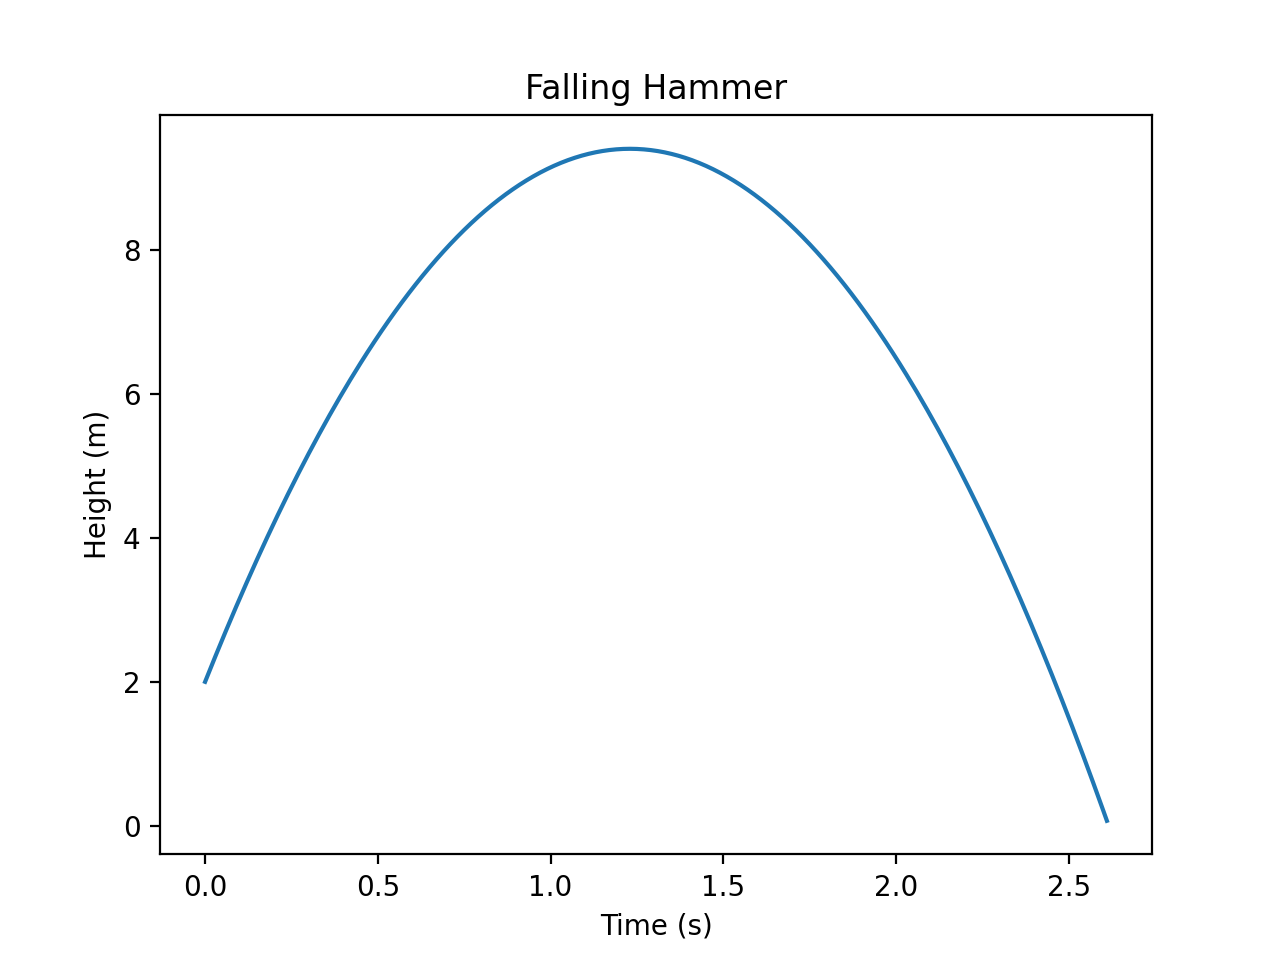
\includegraphics[width=0.7\linewidth]{heightplot.png}

It is more interesting if we can see all three: acceleration, speed, and height. 
So lets make three stacked plots.  Change the plotting code in \filename{falling\_graph.py} to:\index{matplotlib!subplots}

\begin{Verbatim}
# Make a plot with three subplots
fig, ax = plt.subplots(3,1)
fig.suptitle("Falling Hammer")

# The first subplot is acceleration
ax[0].set_ylabel("Acceleration (m/s/s)")
ax[0].plot(times, accelerations)

# Second subplot is speed
ax[1].set_ylabel("Speed (m/s)")
ax[1].plot(times, speeds)

# Third subplot is height
ax[2].set_xlabel("Time (s)")
ax[2].set_ylabel("Height (m)")
ax[2].plot(times, heights)
plt.show()
\end{Verbatim}

Now you will get plots of all three variables:

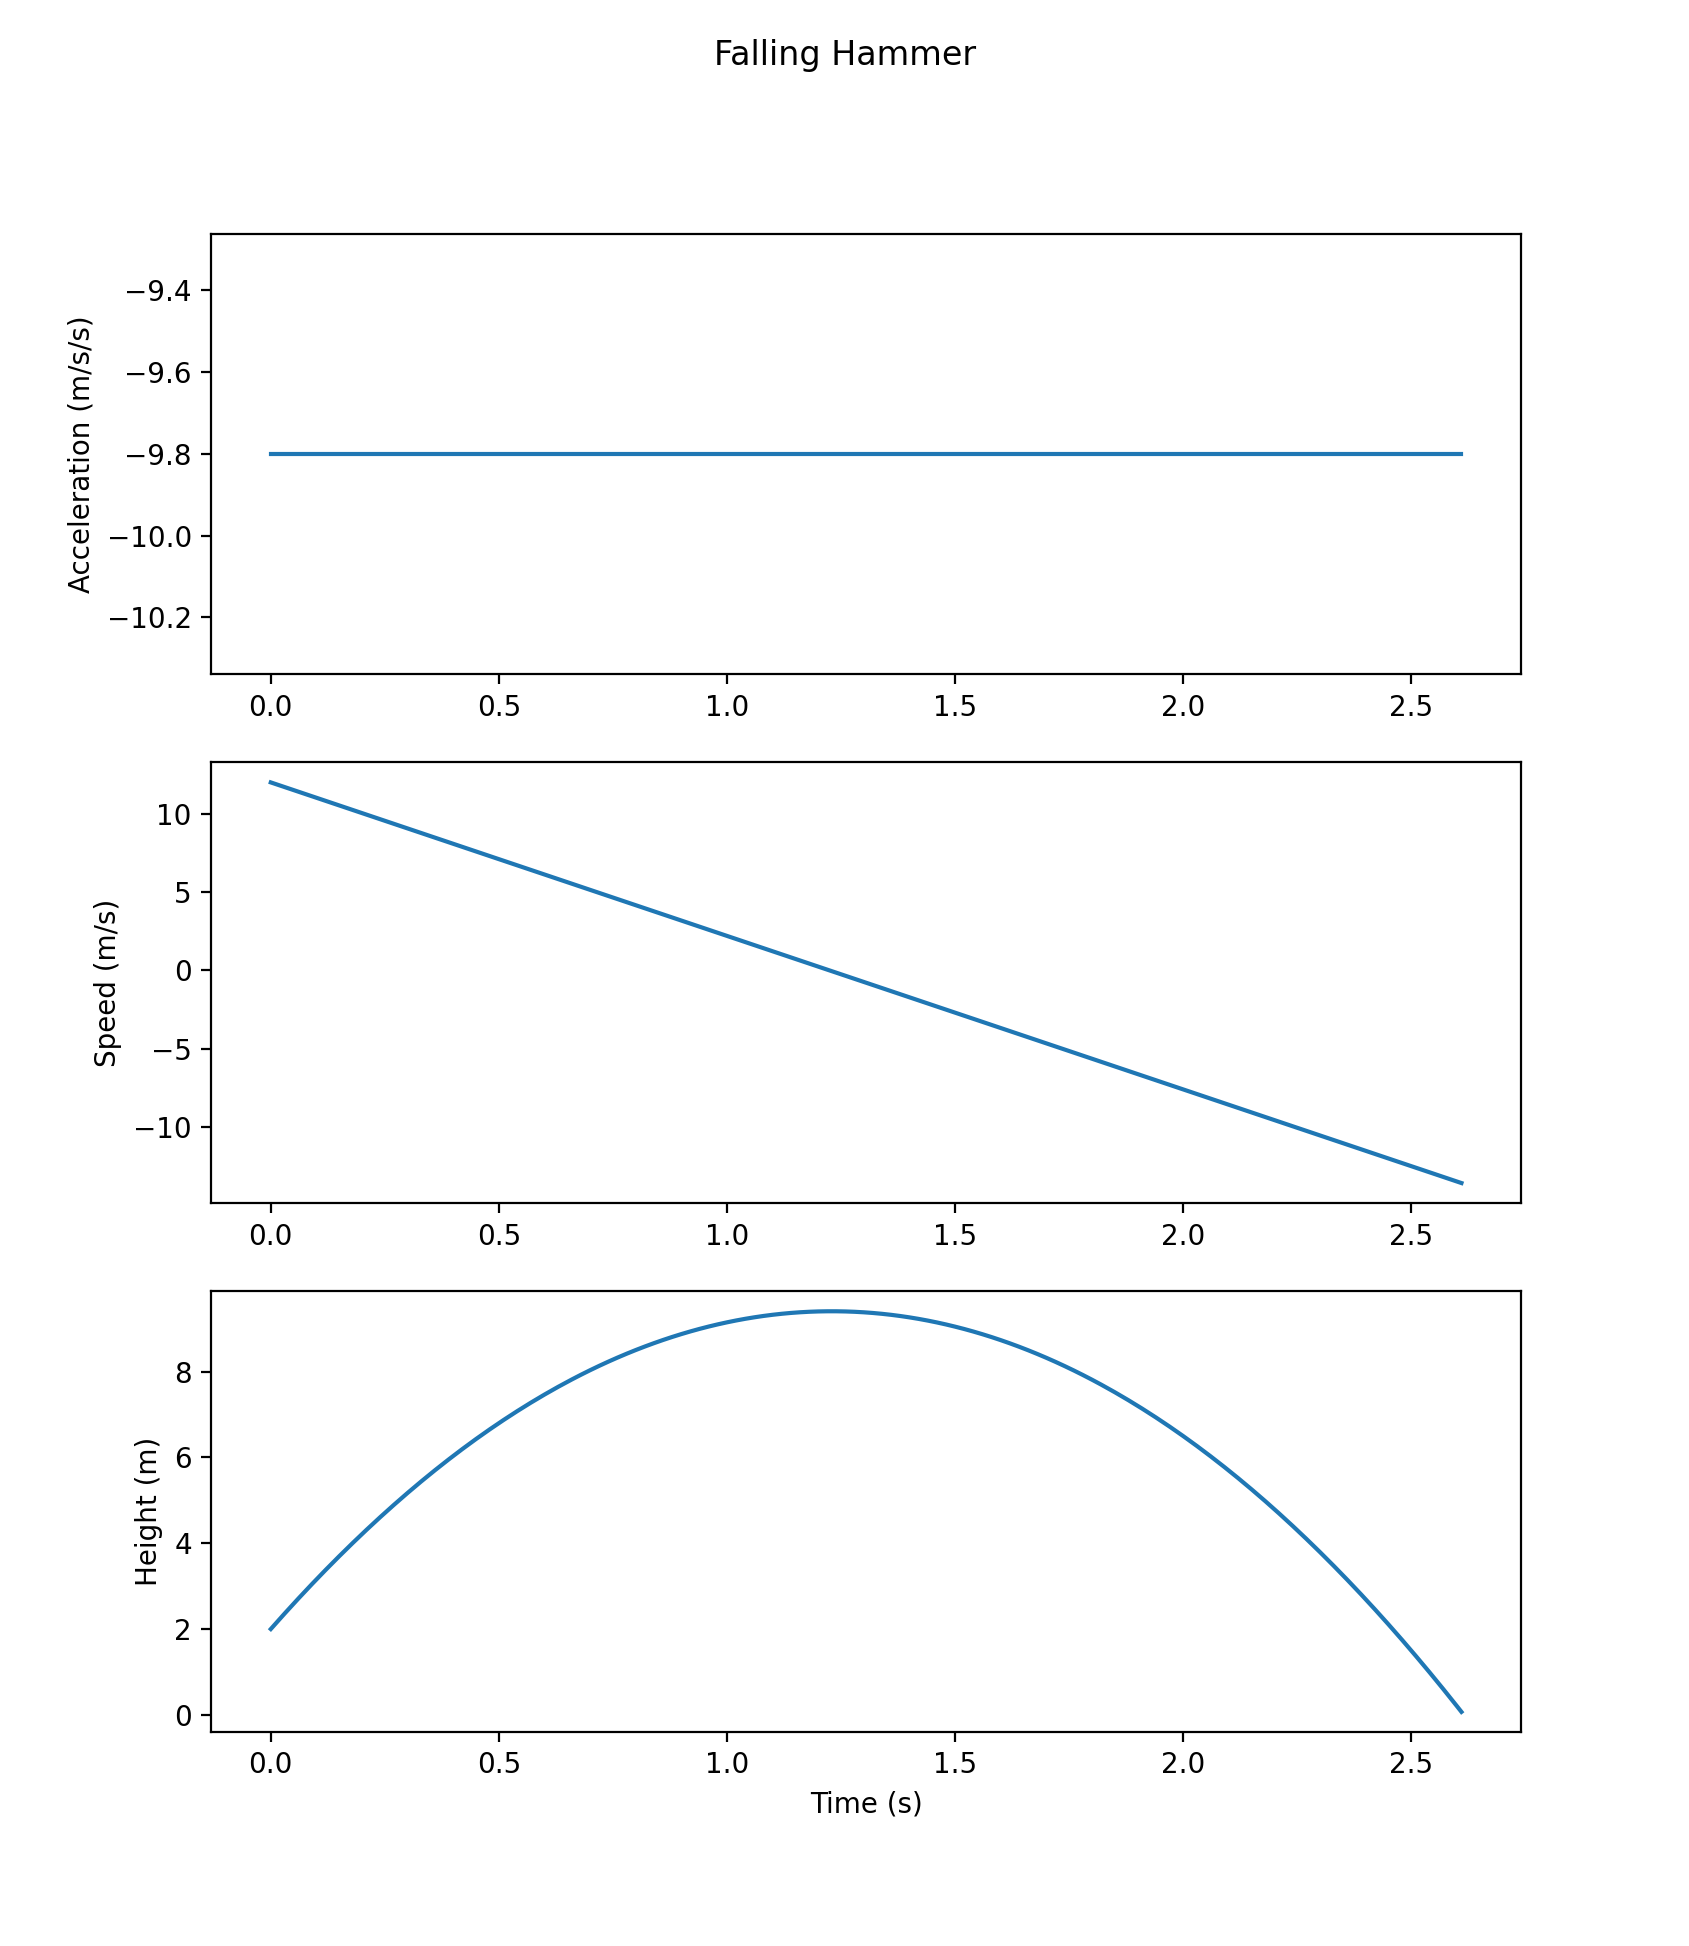
\includegraphics[width=0.8\linewidth]{stackedplot.png}

This is what we expected, right?  The acceleration is a constant negative number.  The speed is a
straight line with a negative slope.  The height is a parabola.

A natural question at this point is ``When exactly will the hammer hit the
ground?''  That is, when does $height = 0$? The values of $t$ where a function is zero are
known as its \textit{roots}. Height is given by a quadratic function. In the next
chapter, you will get the trick for finding the roots of any quadratic
function.

\graphicspath{{../../Chapters/solving_quadratics/en_US}}
\chapter{Solving Quadratics}

A quadratic function has three terms: $ax^2 + bx + c$. $a$, $b$, and
$c$ are known as the \textit{coeffcients}. The coefficients can be any
constant, except that $a$ can never be zero. (If $a$ is zero, it is a linear
function, not a quadratic.)

When you have an equation with a quadratic function on one side and a
zero on the other, you have a quadratic equation. For example:

$$72x^2 - 12x + 1.2 = 0$$

How can you find the values of $x$ that will make this equation true?

You can always reduce a quadratic equation so that the first
coefficient is 1, so that your equation looks like this:

$$x^2 +bx + c = 0$$

For example, if you are asked to solve $4x^2 + 8x - 19 = -2x^2 - 7$
\begin{multline*}
  4x^2 + 8x - 19 = -2x^2 - 7 \\
  6x^2 + 8x -12 = 0 \\
  x^2 + \frac{4}{3}x - 2 = 0
\end{multline*}
Here, $b = \frac{4}{3}$ and $c = -2$.
% This looks a little wonky, maybe add explanations too

\begin{mdframed}[style=important]
$x^2 + bx + c = 0$ when
\begin{equation*}
x = -\frac{b}{2} \pm \frac{\sqrt{b^2 - 4c}}{2}  
\end{equation*}
Only when $a=1$
\end{mdframed}

What does this mean?

For any $b$ and $c$, the graph of $x^2 + bx + c$ is a parabola
that goes up on each end. Its low point is at $x = -\frac{b}{2a}$. This is referred to as the vertex formula.\index{Vertex Formula}

If there are no real roots ($b^2 - 4c < 0$), which means the
parabola never gets low enough to cross the $x$-axis:
\begin{center}
  \begin{tikzpicture}
      \begin{axis}[
          xmin=-0.5,xmax=2.75,
          ymin=-1,ymax=5,
          axis x line=middle,
          axis y line=middle,
          axis line style=<->,
          xlabel={$x$},
          ylabel={$y$},
        ]
        \addplot[no marks,sdkblue] expression[domain=-0.25:2.5,samples=100]{x^2 - 2* x + 3} node[above, xshift=-1cm] {$x^2 - 2x + 3$};
        \addplot[dashed,gray] coordinates {(1,-1)(1,3)};
      \end{axis}
  \end{tikzpicture}
\end{center}

If there is one real root ($b^2 - 4c = 0$), it means that the parabola only touches the x-axis.
\begin{center}
  
  \begin{tikzpicture}
      \begin{axis}[
          xmin=-0.5,xmax=3.75,
          ymin=-0.5,ymax=5,
          axis x line=middle,
          axis y line=middle,
          axis line style=<->,
          xlabel={$x$},
          ylabel={$y$},
        ]
        \addplot[no marks,sdkblue] expression[domain=-0.25:3.5,samples=100]{x^2 - 4*x + 4} node[above, xshift=-1cm] {$x^2 - 4x + 4$};
        \addplot[dashed,gray] coordinates {(2,-0.5)(2,1)};
      \end{axis}
  \end{tikzpicture}
\end{center}

If there are two real roots ($b^2 - 4c > 0$), it means that the parabola crosses the x-axis twice as it dips below and then returns:
\begin{center}
  
  \begin{tikzpicture}
    \begin{axis}[
      xmin=-0.5,xmax=3.75,
      ymin=-2,ymax=5,
      axis x line=middle,
      axis y line=middle,
      axis line style=<->,
      xlabel={$x$},
      ylabel={$y$},
      ]
      \addplot[no marks,sdkblue] expression[domain=-0.25:3.5,samples=100]{x^2 - 3*x + 1} node[above, xshift=-1cm] {$x^2 - 4x + 4$};
      \addplot[dashed,gray] coordinates {(1.5,-2)(1.5,1)};
    \end{axis}
  \end{tikzpicture}
  
\end{center}
\begin{Exercise}[title={Roots of a Quadratic}, label=solve_quadratic]

  In the last chapter, you found that the function for the height of your flying hammer is:

  $$p = -\frac{1}{2}9.8 t^2 + 12t + 2$$

  At what time will the hammer hit the ground?

  
\end{Exercise}
\begin{Answer}[ref=solve_quadratic]

  For what $t$ is  $-4.9 t^2 + 12t + 2 = 0$?  Start by dividing both sides of the equation by -4.9.

  $$t^2 - 2.45 t - 0.408 = 0$$

  The roots of this are at

  $$x = -\frac{b}{2} \pm \frac{\sqrt{b^2 - 4c}}{2} = -\frac{-2.45}{2} \pm \frac{\sqrt{(-2.45)^2 - 4(-0.408)}}{2} = 1.22 \pm 1.36$$

  We only care about the root after we release the hammer ($t > 0$).

  $1.22 + 1.36 = 2.58$ seconds after releasing the hammer, it will hit the ground.

  
\end{Answer}


\section{The Traditional Quadratic Formula}

If the last explanation was a little tricky to understand, the quadratic formula is a nifty tool.

\begin{mdframed}[style=important, frametitle={The Quadratic Formula}]

$ax^2 + bx + c = 0$ when
\begin{equation*}
  x = \frac{-b \pm \sqrt{b^2 - 4ac}}{2a}
\end{equation*}

\end{mdframed}
%FIXME there should be more after this, and an example


\section{Factoring Quadratics}

%FIXME intro section on quadratics, may need some editing and expansion

Sometimes, the quadratic gets a bit clunky and hard so solve, especially without a calculator. That's when factoring quadratics becomes a good tool to use as well.

Factoring quadratics is a way to seperate a quadratic, usually in the form $x^2 + bx + c$ where $(a=1)$, into two multiplied equations in the form $(px + q)(rx + s) = 0$. Solving these for x also gives the roots of the equation. 

\subsection*{Types of Factoring Techniques}

\begin{enumerate}
  \item Factoring out the GCF (Greatest Common Factor) \\
  Always check for a common factor first:
  \[
  2x^2 + 4x = 2x(x + 2)
  \]

  \item Factoring Trinomials: \( a = 1 \) \\
  For expressions like \( x^2 + bx + c \), find two numbers that:
  \begin{itemize}
    \item Multiply to \( c \)
    \item Add to \( b \)
  \end{itemize}
  \[
  x^2 + 5x + 6 = (x + 2)(x + 3)
  \]

  \item Factoring Trinomials: \( a \neq 1 \) \\
  Use the "AC method":
  \begin{enumerate}
    \item Multiply \( a \times c \)
    \item Find two numbers that multiply to \( ac \) and add to \( b \)
    \item Split the middle term and factor by grouping
  \end{enumerate}
  \[
  6x^2 + 11x + 4 = 6x^2 + 3x + 8x + 4 = (3x + 2)(2x + 2)
  \]

  \item Special Cases:
  \begin{itemize}
    \item Perfect Square Trinomials: \\
    \( a^2 + 2ab + b^2 = (a + b)^2 \) \\
    \( x^2 + 6x + 9 = (x + 3)^2 \)

    \item Difference of Squares: \\
    \( a^2 - b^2 = (a - b)(a + b) \) \\
    \( x^2 - 16 = (x - 4)(x + 4) \)
  \end{itemize}
\end{enumerate}

\subsection*{Tips}
\begin{itemize}
  \item Always factor out the GCF first.
  \item Check your result by expanding (FOIL). The inverse of factoring is expanding using the FOIL method.
  \item Not all quadratics are factorable over real integers.
\end{itemize}


%FIXME completing the square section? 

% we should have all 3 factoring methods at least mentioned or taught
\graphicspath{{../../Chapters/complex_numbers/en_US}}
\chapter{Complex Numbers}

Complex numbers are an extension of real numbers, which in turn
are an extension of rational numbers. In mathematics, the set of
complex numbers is a number system that extends the real number line
to a full two dimensions, using the imaginary unit, which is denoted by
$i$, with the property that $i^2 = -1$.\index{Complex Numbers}

An imaginary number is a number that is a multiple of the imaginary unit $i$.
For example, $5i$ and $-3i$ are both imaginary numbers. While imaginary numbers are a 
subset of complex numbers (with real part equal to zero), not all complex numbers are 
imaginary. Complex numbers can have both a real and an imaginary part, while imaginary 
numbers specifically refer to those with no real part.

\section{Definition}

A complex number is a number of the form $a + bi$, where $a$ and $b$
are real numbers, and $i$ is the imaginary unit, with the property
that $i^2 = -1$. The real part of the complex number is $a$, and the
imaginary part is $bi$.

\section{Why Are Complex Numbers Necessary?}

Complex numbers are essential to many fields of science and
engineering. Here are a few reasons why:

\subsection{Roots of Negative Numbers}

In the real number system, the square root of a negative number does
not exist, because there is no real number that you can square to get a
negative number. The introduction of the imaginary unit $i$, which has
the property that $i^2 = -1$, allows us to take square roots of
negative numbers and gives rise to complex numbers.

\subsection{Polynomial Equations}

The fundamental theorem of algebra states that every non-constant
polynomial equation with complex coefficients has a complex root. This
theorem guarantees that polynomial equations of degree $n$ always have
$n$ roots in the complex plane.

\subsection{Physics and Engineering}

In physics and engineering, complex numbers are used to represent
waveforms in control systems, in quantum mechanics, and many other
areas. Their properties make many mathematical manipulations more
convenient.

\section{Adding Complex Numbers}

The addition of complex numbers is straightforward. If we have two
complex numbers $z_1 = a + bi$ and $z_2 = c + di$, their sum is
defined as:

\begin{equation}
z_1 + z_2 = (a + c) + (b + d)i
\end{equation}

In other words, you add the real parts to get the real part of the
sum, and add the imaginary parts to get the imaginary part of the sum.

\section{Multiplying Complex Numbers}

The multiplication of complex numbers is a bit more involved. If we
have two complex numbers $z_1 = a + bi$ and $z_2 = c + di$, their
product is defined as:

\begin{equation}
z_1 \cdot z_2 = (a + bi) \cdot (c + di) = ac + adi + bci - bd = (ac - bd) + (ad + bc)i
\end{equation}

Note the last term comes from $i^2 = -1$. You multiply the real parts
and the imaginary parts just as you would in a binomial
multiplication, and remember to replace $i^2$ with $-1$. See the Khan academy video
in the digital resources for a more in-depth explanation.


%%%%%%%%%%%%%%%%%%%%%%%%%%%%%%%%%
%% Bookfooter.tex by Aaron Hillegass
%% Nov 8, 2020

\appendix

\chapter{Answers to Exercises}
\shipoutAnswer

\bibliography{references}

\printindex

\end{document}